\section{abstract}
Lorem ipsum dolor sit amet, consectetur adipiscing elit. Nam a orci ornare nibh tincidunt molestie sed nec tellus. Morbi non sapien id lorem posuere pretium. Vestibulum commodo cursus purus, a elementum sem imperdiet sit amet. Phasellus posuere dolor dignissim aliquam tempus. Morbi egestas felis in lorem varius, ac egestas ante lacinia. Nulla sed ultrices dui. Lorem ipsum dolor sit amet, consectetur adipiscing elit. 

\section{Introduction}

Bitcoin ~\cite{nakamoto2008bitcoin} emerged less than a decade ago as an open source project, which mushroomed to an industry worth more than 250 billion dollars as of this report's writing (Global Charts - CoinMarketCap https://coinmarketcap.com/charts/), which is made up of many different cryptocurrencies. Consequently, every day people new to the concept of cryptocurrencies look for a quick and simple way to acquire some crypto wealth. In the early days many decided to speed up the process of mining for themselves by combining CPUs and GPUs to work together. Other groups of people deployed snippets of JavaScript code on websites that recruited their visitors’ CPU power, often unknowingly, to mine for them as part of a bigger mining network (a.k.a botnet). However, both approaches quickly became infeasible as the computing power required to mine bitcoins grew exponentially to over 12 petahashes/s (Hash Rate - Blockchain https://blockchain.info/charts/hash-rate), and lead to the emergence of application-specific integrated circuits (ASICs) and collective mining pools to continue the mining race. As the years passed and a few key cryptocurrencies emerged as the market leaders, the concept of in-browser crypto-mining largely became forgotten. Today, the most common way for the average person to acquire cryptocurrencies is to purchase them. Unusually, stories began to circulate on popular media outlets this year of websites mining cryptocurrencies through browsers again. And even more intriguingly, high profile websites were now involved, and the practice seemed to be growing at a quick pace.

\begin{center}
	\makebox[1\textwidth]{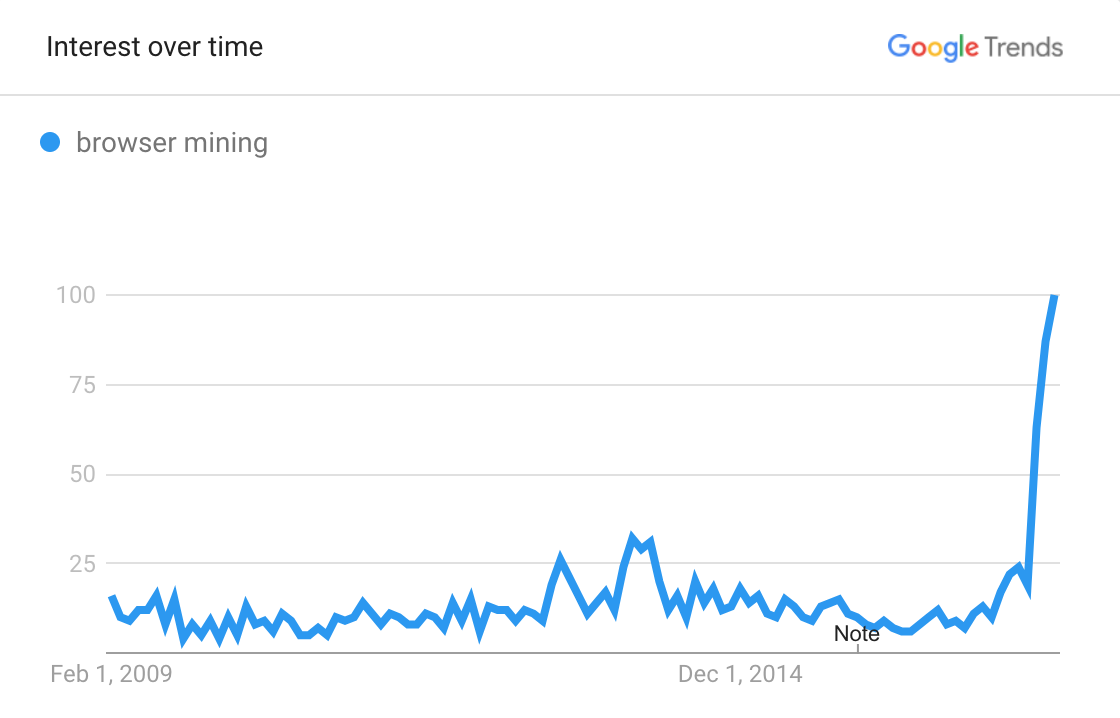
\includegraphics[width=1\textwidth]{browser_mining.png}}
	\caption{Search interest for "browser mining" over time}
\end{center}

The graph above shows how the searches for "browser mining" have changed since Bitcoin was launched. Search interest seems to have piqued during price surges, which culminated with Bitcoin crossing $1000 USD. Soon after Bitcoin's first major crash, searches consistently waned until a recent large spike that is more than 4 times the lifetime average. The waning period before the recent surge could be attributed to the advent of ASIC usage for Bitcoin mining, and the surge is likely due to the revival of browser mining for non-Bitcoin currencies that have gained a sizeable market capitalization. As a result, websites like Showtime.com (Showtime websites secretly mined user CPU for cryptocurrency - The Verge https://www.theverge.com/2017/9/26/16367620/showtime-cpu-cryptocurrency-monero-coinhive), and ThePirateBay.org (Browser-Based Mining Malware Found on Pirate Bay, Others - ExtremeTech https://www.extremetech.com/internet/255971-browser-based-cryptocurrency-malware-appears-online-pirate-bay) have been experimenting with in-browser mining as a way to add a new revenue stream.

\section{Egalitarian Proof-of-Work}

One of the reasons for the resurgence of this type of mining is the recent rise in price and popularity of the cryptocurrency Monero ~\cite{monero}. Launched in April 2014, Monero focuses on privacy by obfuscating the participants and amounts in transactions. This is in contrast to more popular cryptocurrencies like Bitcoin and Ethereum where transactions can be traced back through the entire blockchain. In fact, Monero gained some fame for its ability to anonymize bitcoins by converting them into Monero, transacting them privately, and then converting them back to bitcoins. This has made Monero popular on black market websites where illicit goods can be purchased without having transactions traced back to buyers. 
\\
More importantly, Monero differs in the way its currency is mined by employing a proof-of-work that is egalitarian by design. This is achieved by using the proof-of-work algorithm named CryptoNight **CITATION**, which makes its puzzle resistant to ASICs and fast memory-on-chip devices with low latency. While many cryptocurrencies use a similar type of proof-of-work, Monero was one of the earliest to adopt and popularize it. 
\\
Bitcoin uses SHA-256 for its hash-based proof-of-work algorithm, which is a CPU-bound function. This allows miners to use ASIC devices to increase their calculation speeds, which greatly surpasses an ordinary computer in hashes per unit of money. CryptoNote, which is an evolution of Bitcoin that acts as the application layer protocol to power several cryptocurrencies such as Monero, chose CryptoNight for its proof-of-work. CryptoNight uses a memory-bound function, which relies on a situation where the time taken to complete a given computational problem is decided primarily by the amount of memory required to hold data. This limits the ability for pipelining, which is also known as instruction-level parallelism.  
\\
Satoshi Nakamoto’s original philosophy and intention for Bitcoin was “one-CPU-one-vote” **CITATION**, which CryptoNight attempts to enforce. In CryptoNight, users vote for the right order of transactions and honest money supply distribution with their CPU power, so the more CPU cores they have the more voting power they acquire. Since CPUs are relatively affordable and accessible, it follows that most users will have approximately equal voting rights. Then by relying on random access to a slow memory and emphasizing latency dependence, it is ensured that proof-of-work is largely controlled by CPUs instead of GPUs and ASICs. This is done by having every new block depend on the previous block’s solution, which must be kept in memory. This algorithm requires approximately 2MB per instance, which fits in the L3 cache per core of modern processors. Over the course of the next few years, these modern processor L3 cache sizes should become mainstream and allow more CPUs, and thus users, to vote in the Monero ecosystem. It has also been shown that ASICs cannot handle more than 1MB of internal memory, which is less than the size of memory required to calculate a new block. GPUs are also at a disadvantage since GDDR5 memory, for example, is notably slower than L3 cache. **CITATION** 
\\

4. Significant expansion of the scratchpad would require an increase in iterations, which in turn implies an overall time increase. "Heavy" calls in a trust-less p2p network may lead to serious vulnerabilities, because nodes are obliged to check every new block's proof-of-work. If a node spends a considerable amount of time on each hash evaluation, it can be easily DDoSed by a flood of fake objects with arbitrary work data (nonce values).
\\
While Monero is a good choice as cryptocurrency for in-browser mining, several improvements can be suggested to make it more ideal. %depending if this falls in our scope. we can mention this in future work or conclusion, just for the sake of having it.


\section{Browser Mining}

% History of browser mining goes here
In the early days of cryptocurrency mining, there was a rise of Bitcoin javascript miners such as JSMiner (2011) and MineCrunch (2014). Minecrunch had a bigger campaing and more online presents by their developer. Based on what the developer claimed, the javascript miner was optimised and worked 1.5x slower than native CPUMiner. However as the hashing power of Bitcoin network increased, the mining difficulty increased and Bitcoin CPU mining was not profitable any more, hence the developers stopped maintaining the code base of such miners.   

%Some examples on coinhive website such as Shortlinks, Captcha , ... 
**INTRODUCE COIN-HIVE, AND WHY WE FOCUSED ON IT INSTEAD OF OTHERS LIKE COIN-LOOT**
** NEEDS MORE HERE ** 

\section{Experiment}

Assumptions
	We start our experiment by some assumptions based on our knowledge of how this process would affect users, and we will revisit these assumptions with the result from our experiments.
We will track three different measurements:
CPU Usage percentage over a period of time on a webpage
Miner off
Miner on
Electricity Usage (Battery drain on mobile devices)
Network Usage over a period of time on a webpage
Miner off
Miner on
We will do these experiments on different devices, such as a Laptop, a PC, an Android phone and an iPhone, …

\begin{center}
	\makebox[1\textwidth]{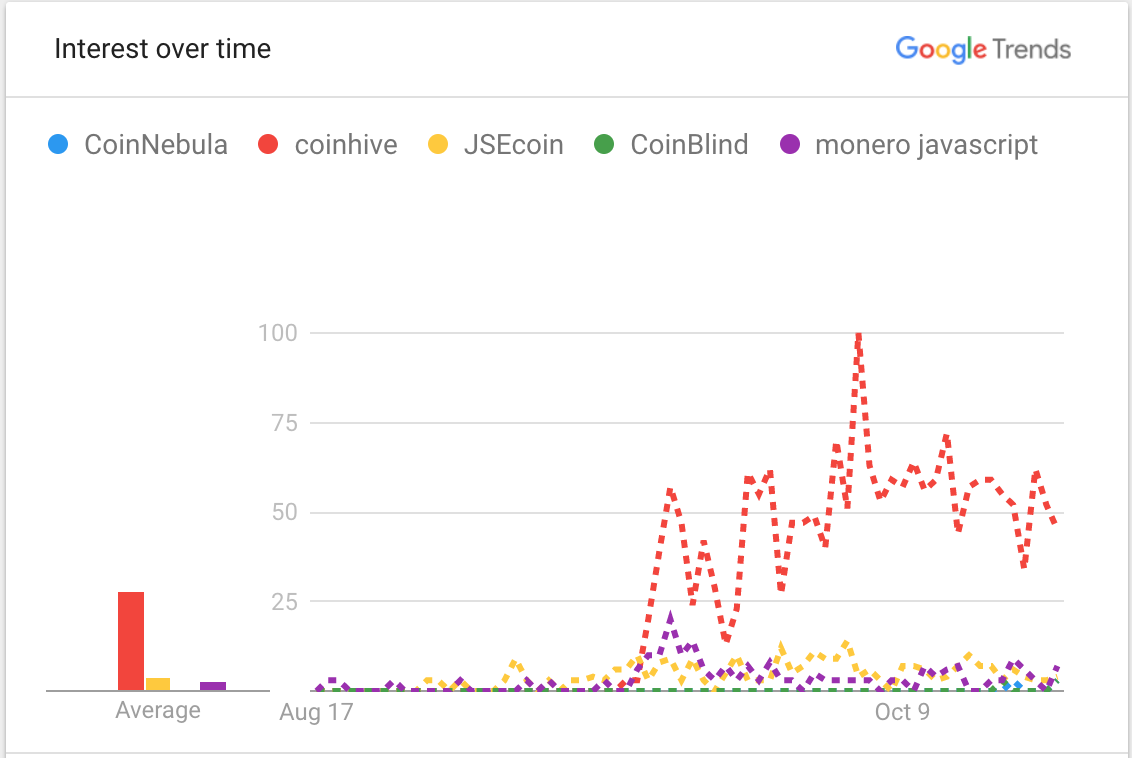
\includegraphics[width=1\textwidth]{usage_over_time.png}}
\end{center}


Our hypotheses are that the CPU usage and electricity usage will be heavily affected by running the miner on the webpage. As for Network usage, our estimation is that there will be more traffic when miners are running, but no conclusion about the impact can be made at this time.


\section{User Impact}

Most in-browser crypt-minings are running without the consent, nor knowledge, of the users involved. The websites that have been found to be running JavaScript code for the purpose of mining usually employ the API from a startup named Coin-Hive~\cite{coinhive}. One such website, for example, is the website PirateBay.org **CITATION** that now runs the JavaScript code when searching for torrent files. Perhaps unsurprisingly, there is no notice in their Privacy Policy nor visible warning on any part of the website that informs their users of this activity. This is in contrast to the banners users are presented with upon the first visit to a website that warns them of the website’s policy on cookies **MAYBE SOMETHING ABOUT EU LAW ON THIS?**. It’s now widely known that these cookies can be used to track users across the internet, so cookie banners can act as a reminder and allow the user to make better informed decisions regarding their browsing habits. Without any type of disclaimer for users, websites admins are commandeering their users’ CPU resources for their business or personal gain. This results in higher energy bills for the user, along with accelerated device degradation, and slower system performance.
\\
A second example of a popular website deploying Coin-Hive’s API is Showtime.com **CITATION**, which is a popular cable channel that also streams their TV shows online. It then came as no surprise when UFC.com was accused of using this very same code on the night of one of their most popular events **CITATION**. This trend of websites that offer streaming services deploying Coin-Hive’s API could be due to the high costs of providing streaming. While ads can be used to offset some of the costs, it would be of interest to some to at least experiment with the idea of recruiting their users to mine Monero, which can be sold later.
\\
The opinion of the authors of this report maintain that users should be given the option to enable this JavaScript code with some benefit to them.  An example of a benefit could be the removal of ads. Another example would be granting access to premium features of the website such as journal articles behind a paywall, or streaming in high-definition. The website could also allow the user to participate in block rewards by allocating a large portion of their CPU resources to the activity of mining, which would benefit both parties. By notifying the user of the potential of this activity, and allowing them to make a choice to participate, the website maintains trust in the relationship with the user while also benefiting from a new source of revenue. By foregoing disclaiming this new activity that can have harmful effects, the website will only gain a new revenue stream for a short time while sacrificing their reputation. Coin-Hive’s recent response to the market’s negative reaction, which included blocking their extension, was to release a new feature called AuthedMine, that would enforce user consent before enabling of any mining JavaScript code. 
\\
We also see the potential for this new form of revenue generation to compete with advertisements, and perhaps one day replace them. This is because the malware that is associated with advertisements is still a growing concern, and the public’s dislike of advertisements will persist and never wane. Also, as cryptocurrencies continue to grow in market capitalization and use cases, their inevitable mainstream use will push the profitability of egalitarian proof-of-work cryptocurrencies such as Monero well into the future.

\begin{center}
	\makebox[1\textwidth]{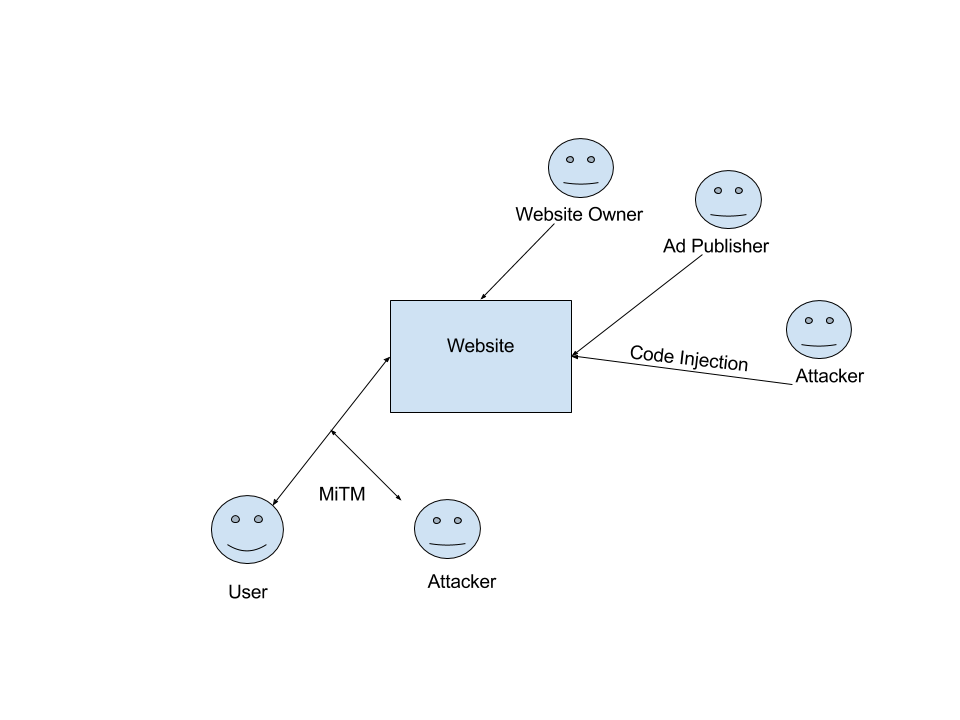
\includegraphics[width=1\textwidth]{attack_vectors.png}}
\end{center}

\section{Discussion}
Future possibilities:
	- every website uses a browser miner. if many tabs are open, how are user's CPU resources shared? first tab takes all the CPU 		power, or is it shared evenly? Can that remain profitable for websites? will that cause too much strain on the user's CPU?
	- would users be happy with giving some of their idle CPU to websites? if so, how much? would they change their minds if battery 	was impacted too severely?
	- should this be implemented at OS level?
	- Facebook/Google have a duopoly on the market and control prices (>60 percent of revenue from ads), so would this be 			competitive for websites?

\section{Conclusion}
In conclusion, the use of in-browser crypto-mining is a growing trend among websites that rely on generating website visits by offering video streaming or online gambling. The deployment of Coin-Hive’s API, and others like it, is a low-risk experiment for some high-profile websites that seek to validate the concept of recruiting their users’ CPU power to mine egalitarian proof-of-work cryptocurrencies. If, as we have determined, the model can be proven to be financially viable, this type of JavaScript code may become widespread in a short period of time. However, this will rely on the consent of users that will either be enforced through new regulations or proper ethical etiquette from leading internet companies and startups. If the proper steps are not taken, then this mining technique may be used illicitly in the form of botnets or individually by unscrupulous websites. The result will be higher energy bills for victims, along with slower system performance and accelerated device degradation.
